\begin{figure}[h!]
    \centering
    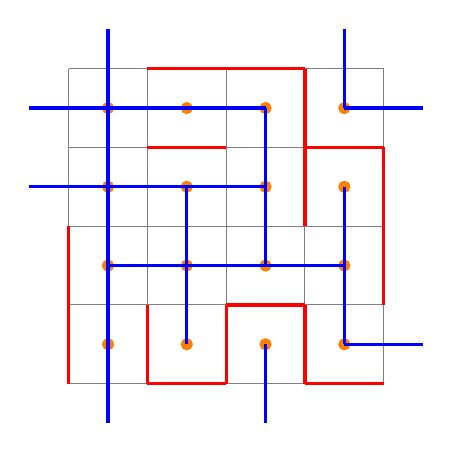
\begin{tikzpicture}
        % Grid
        \foreach \x in {0, 1, ..., 4} {
            \draw[gray] (0, \x) -- (4, \x);
            \draw[gray] (\x, 0) -- (\x, 4);
        }
        
        
        \foreach \i in {0.5, 1.5, ..., 3.5} {
            \foreach \j in {0.5, 1.5, ..., 3.5} {
                \filldraw[orange] (\i, \j) circle (2.0pt);
            }
        }
        
        % Percolation
        %% |
        \draw[red, very thick] (0, 2) -- (0, 0);
        \draw[red, very thick] (1, 1) -- (1, 0);
        \draw[red, very thick] (2, 1) -- (2, 0);
        \draw[red, very thick] (3, 4) -- (3, 2); 
        \draw[red, very thick] (3, 1) -- (3, 0);
        \draw[red, very thick] (4, 3) -- (4, 1);
        %% -
        \draw[red, very thick] (1, 4) -- (3, 4);
        \draw[red, very thick] (1, 3) -- (2, 3);
        \draw[red, very thick] (3, 3) -- (4, 3);
        \draw[red, very thick] (2, 1) -- (3, 1);
        \draw[red, very thick] (1, 0) -- (2, 0);
        \draw[red, very thick] (3, 0) -- (4, 0);
        
        % Dual percolation
        %% -
        \draw[blue, very thick] (-0.5, 3.5) -- (2.5, 3.5);
        \draw[blue, very thick] (3.5, 3.5) -- (4.5, 3.5);
        \draw[blue, very thick] (-0.5, 2.5) -- (2.5, 2.5);
        \draw[blue, very thick] (0.5, 1.5) -- (3.5, 1.5);
        \draw[blue, very thick] (3.5, 0.5) -- (4.5, 0.5);
        %% |
        \draw[blue, very thick] (0.5, 4.5) -- (0.5, -0.5);
        \draw[blue, very thick] (1.5, 2.5) -- (1.5, 0.5);
        \draw[blue, very thick] (2.5, 3.5) -- (2.5, 1.5);
        \draw[blue, very thick] (2.5, 0.5) -- (2.5, -0.5);
        \draw[blue, very thick] (3.5, 4.5) -- (3.5, 3.5);
        \draw[blue, very thick] (3.5, 2.5) -- (3.5, 0.5);
        
    \end{tikzpicture}
    \caption{A percolation realisation on a $5 \times 5$ section of the square lattice and its dual}
    \label{fig:square_lattice_dual}
\end{figure}